\documentclass{techbrief}

\usepackage{tikz, pgfplots}
\usetikzlibrary{positioning,calc,arrows,arrows.meta, shapes, decorations.markings}
\usetikzlibrary{decorations.pathreplacing}


\title{The Born rule is equivalent to the von Neumann entropy}
\author{Gabriele Carcassi}
\category{Quantum mechanics}
\tags{Born rule, Entropy}

\begin{document}
	
\maketitle
	
\begin{abstract}
	We show that the Born rule in quantum mechanics coincides with the definition of entropy. That is, assuming that conditional probability is given by the Born rule is equivalent to as assuming that the entropy is given by the von Neumann entropy.
\end{abstract}

\section{Introduction}

In quantum mechanics, the Born rule
\begin{equation}
	p(\psi|\phi) = \frac{\< \phi | \psi \>\< \psi | \phi \>}{\< \psi | \psi \>\< \phi | \phi \>}
\end{equation}
defines conditional probability for two states: the probability of measuring state $\phi$ given that $\psi$ was prepared. Similarly, the von Neumann entropy
\begin{equation}
	S(\rho) = - \tr(\rho \log \rho)
\end{equation}
defines the entropy for quantum ensembles. Here we show that any of the two can be defined on top of the other, meaning that they impose the same structure.

\section{Core insight}

Let us first show that, once the full framework of quantum mechanics is assumed, there is an invertible function between the Born rule and the entropy of equal mixtures of two states.

\begin{prop}[Born rule is entropy]\label{QM-ENT-PROB}
	Let $\psi, \phi \in P[\mathcal{H}]$ be two quantum states. The probability of measuring $\phi$ having prepared $\psi$ is uniquely determined by the entropy of their equal mixture and vice versa. More precisely, $p(\phi|\psi) = \lambda$ if and only if $S\left(\frac{1}{2} \rho_{\psi} + \frac{1}{2} \rho_{\phi} \right) =  - \frac{1+\sqrt{\lambda}}{2} \log \frac{1+\sqrt{\lambda}}{2} - \frac{1-\sqrt{\lambda}}{2} \log \frac{1-\sqrt{\lambda}}{2}.$
\end{prop}

\begin{figure}[h]
	\centering
	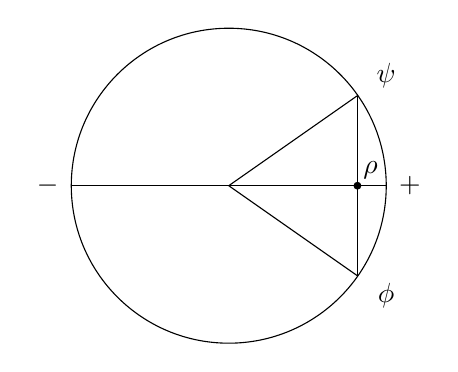
\begin{tikzpicture}[scale = 1]
		\draw (0,0) circle (2);
		\node at (-2.3,0) {$-$};
		\node at (2.3,0) {$+$};
		\node at (2,1.4) {$\psi$};
		\node at (2,-1.4) {$\phi$};
		\draw (-2,0) -- (2,0);
		\begin{scope}
			\clip(0,0) circle (2);
			\draw (0,0) -- (2,1.4);
			\draw (0,0) -- (2,-1.4);
			\draw (1.634,1.4) -- (1.634,-1.4);
		\end{scope}
		\fill (1.634,0) circle (0.05);
		\node at (1.8,.2) {$\rho$};
	\end{tikzpicture}
	\caption{Geometric diagonalization of an equal mixture of two states.}\label{rp-qm-geometricDiagonalization}
\end{figure}

\begin{proof}
	We want to show that there exists an invertible relationship between the Born rule and the entropy for equal mixtures of two states. To gain better insight, let us construct the proof geometrically as in Fig. \ref{rp-qm-geometricDiagonalization}. Let $\psi$ and $\phi$ be two pure states. Their equal mixture $\rho=\frac{1}{2}\rho_{\psi} + \frac{1}{2}\rho_{\phi}$ will be the midpoint between them. To calculate the entropy, we need to diagonalize $\rho$ and calculate the Shannon entropy from the eigenvalues. To diagonalize $\rho$ we need to express it as a mixture of two orthogonal states $+$ and $-$. But $+$ and $-$ will be orthogonal only if they are opposite points on the Bloch sphere. Therefore, $\rho$ is diagonalized by $+$ and $-$ if and only if it lies on the axis identified by $+$ and $-$ as we see in Fig. \ref{rp-qm-geometricDiagonalization}. Geometrically, we will have $\rho = \frac{\overline{-\rho}}{\overline{-+}}\rho_{+} + \frac{\overline{\rho+}}{\overline{-+}}\rho_{-}$. Using trigonometry we have:
	\begin{equation}
		\begin{aligned}
			\rho &= \frac{\overline{-\rho}}{\overline{-+}}\rho_{+} + \frac{\overline{\rho+}}{\overline{-+}}\rho_{-} = \frac{1+\cos \theta_{\psi+}}{2}\rho_{+} + \frac{1-\cos \theta_{\psi+}}{2}\rho_{-}.
		\end{aligned}
	\end{equation}
	
	Now recall that, geometrically, the Born rule represents the cosine square of the half-angle between two states. That is,
	\begin{equation}
		\begin{aligned}
			p(\psi|\phi) &= \frac{\< \phi | \psi \>\< \psi | \phi \>}{\< \psi | \psi \>\< \phi | \phi \>} = \cos^2 \frac{\theta_{\psi\phi}}{2} = \cos^2 \theta_{\psi+} \\
			\rho &= \frac{1+\sqrt{p(\phi|\psi)}}{2}\rho_{+} + \frac{1-\sqrt{p(\phi|\psi)}}{2}\rho_{-}.
		\end{aligned}
	\end{equation}
	
	Since $+$ and $-$ are orthogonal, the entropy of $\rho$ is
	\begin{equation}
		\begin{aligned}
			S(\rho) = - \tr(\rho \log \rho) = - \frac{1+\sqrt{p(\phi|\psi)}}{2} \log \frac{1+\sqrt{p(\phi|\psi)}}{2} - \frac{1-\sqrt{p(\phi|\psi)}}{2} \log \frac{1-\sqrt{p(\phi|\psi)}}{2}.
		\end{aligned}
	\end{equation}
	
	\begin{figure}[h]
		\centering
		\begin{tikzpicture}
			\def\xi{0.25};
			\def\vi{1.25};
			\def\m{1};
			\def\b{1};
			\pgfplotsset{ticks=none}
			\begin{axis}[
				width=5.3cm,
				height=4.5cm,				
				axis lines=middle,
				axis line style={-},
				clip=false,
				xlabel=$p(\phi | \psi)$,
				xlabel style={below=5pt},
				ylabel=$S\left(\frac{1}{2} \rho_{\phi} + \frac{1}{2} \rho_{\psi}\right)$,
				ylabel style={above=2pt, left},
				xmin=0,xmax=1.1,
				ymin=0,ymax=0.8,
				domain=0:4,
				]
				\addplot[black,samples=69]{ - ((1+sqrt(x))/2) * ln((1+sqrt(x))/2) - ((1-sqrt(x))/2) * ln((1-sqrt(x))/2)}
				node [pos=0,left] {$1$};
			\end{axis}
		\end{tikzpicture}
		\caption {Entropy of a mixture of two pure states as a function of their Born rule.} \label{fig_rp_qm_entropyVsProb}
	\end{figure}
	The relationship is plotted in Fig. \ref{fig_rp_qm_entropyVsProb}: it is strictly concave and, therefore, invertible. If we are given the entropy of all equal mixtures of pairs of states we would be able to recover the Born rule and vice-versa.
\end{proof}

\begin{coro}[Orthogonality is mutual exclusivity]\label{rp-qm-orthoIsMutex}
	Given $\psi, \phi \in P[\mathcal{H}]$, $\<\phi|\psi\> = 0 \iff p(\phi | \psi) = 0 \iff S\left(\frac{1}{2} \rho_{\psi} + \frac{1}{2} \rho_{\phi} \right) = 1$.
\end{coro}

\section{Premises and conditions}

We now want to state the overall claim in terms of dependency of definitions.

The following condition represents our base theory, and defines the space of ensembles together with basic necessary requirements for conditional probability and entropy.

\begin{condition}[Ensembles and quantum states]{EQST}
	The space of ensembles $E(\mathcal{H}$) of a quantum system is represented by the convex space of all density operators (i.e positive semi-definite trace one self-adjoint operators) over a suitable separable inner product space $\mathcal{H}$. The state space is the set of extreme points, which coincides with the projective space $P(\mathcal{H})$. The ensemble space is equipped with a function $S : E(\mathcal{H})$ where $S(\rho)$ returns the entropy for ensmble $\rho$. The ensemble space is also equipped with a function $p(\cdot | \cdot) : P(\mathcal{H}) \times E(\mathcal{H}) \to [0,1]$, where $p(\psi | \rho)$ returns the probability of finding $\psi$ having prepared $\rho$. This function is affine in the second argument (i.e. $p(\phi | \sum p_i \psi_i) = \sum_i p_i p(\phi | \psi_i)$ ) and returns one if and only if the initial and final states are the same (i.e. $p(\phi | \psi) = 1 \iff \phi = \psi$ for all $\psi, \phi \in P(\mathcal{H})$).
\end{condition}

\begin{coro}
	Since every ensemble $\rho$ can be expressed as the convex combination of pure states, function $p$ is fully specified by its values on pure states.
\end{coro}

The following condition links the inner product to the conditional probability.

\begin{condition}[Born rule]{BR-BORN}
	The conditional probability $p$ is given by the Born rule: $p(\psi|\phi) = \frac{\< \phi | \psi \>\< \psi | \phi \>}{\< \psi | \psi \>\< \phi | \phi \>}$.
\end{condition}

The following condition imposes that the entropy is the von Neumann entropy.

\begin{condition}[Von Neumann entropy]{BR-ENT}
	The entropy function $S$ is given by the Shannon entropy: $S(\rho) = \tr(\rho \log \rho)$.
\end{condition}

The following condition makes sure that mutual exclusivity is consistently defined across conditional probability and entropy.

\begin{condition}[Mutual exclusivity conditions]{MUTEX}
	Let $\psi_i \in P(\mathcal{H})$ be a countable sequence of states. Then $p(\psi_i | \psi_j) = 0$ for all $i \neq j$ if and only if $S(\sum_i p_i \psi_i) = - \sum_i p_i \log p_i$ for all $p_i$ such that $\sum_i p_i = 1$.
\end{condition}

\begin{thrm}
	Over \ref{EQST}, if two conditions among \ref{BR-BORN}, \ref{BR-ENT} and \ref{MUTEX} are assumed, the third is implied.
\end{thrm}

\begin{proof}
	Let us show that \ref{BR-BORN} and \ref{BR-ENT} imply \ref{MUTEX}. Given a sequence of states $\psi_i \in P(\mathcal{H})$, we can find a sequence of normalized representatives $|\psi_i\>$. Suppose $\psi_i$ are pairwise orthogonal, then $|\psi_i\>$ are orthogonal as well. Let $\rho = \sum_i p_i \psi_i$. Then $ - \rho \log \rho = - \sum_i p_i \log p_i \psi_i$ and $-\tr(\rho \log \rho) = - \sum_i p_i \log p_i$. Conversely, suppose $|\psi_i \>$ is a sequence of normalized representatives of not necessarily pairwise orthogonal states. Since $S(\sum_i p_i \psi_i) = - \sum_i p_i \log p_i$ for all $p_i$ such that $\sum_i p_i = 1$, in particular we will have $S\left(\frac{1}{2} \rho_{\psi_i} + \frac{1}{2} \rho_{\phi_j} \right) = 1$ for all $i \neq j$. By \ref{rp-qm-orthoIsMutex}, $p(\psi_i|\psi_j) = 0$ for all $i \neq j$.
	
	Let us show that \ref{BR-BORN} and \ref{MUTEX} imply \ref{BR-ENT}. Given an ensemble $\rho \in E(\mathcal{H})$ we can find a sequence of orthogonal states $\psi_i$ such that $\rho = p_i \psi_i$. Since they are orthogonal, by \ref{BR-BORN} we have $p(\psi_i|\psi_j) = \frac{\< \psi_i | \psi_j \>\< \psi_j | \psi_i \>}{\< \psi_i | \psi_i \>\< \psi_j | \psi_j \>} = 0$ for all $i \neq j$. By \ref{MUTEX}, $S(\rho) = - \sum_i p_i \log p_i = - \tr(\sum_i p_i \log p_i \psi_i) = - \tr(\rho \log \rho)$.
	
	Let us show that \ref{BR-ENT} and \ref{MUTEX} imply \ref{BR-BORN}. Let $\psi, \phi \in P(\mathcal{H})$. By the same arguments used in the proof of \ref{rp-qm-geometricDiagonalization}, $\< \phi | \psi \> = 0$ if and only if $S\left(\frac{1}{2} \rho_{\psi} + \frac{1}{2} \rho_{\phi} \right) = 1$ and, by \ref{MUTEX}, if and only if $p(\phi | \psi) = 0$. Therefore, we recover the idea that orthogonality from the inner product corresponds to mutual exclusivity in terms of conditional probabilities. Now, let $\psi, \phi \in P(\mathcal{H})$ not necessarily orthogonal, and let $V \subseteq E(\mathcal{H})$ be the convex set of all ensembles that have support on the subspace defined by the span of $\psi$ and $\phi$. This will be a Bloch ball and will contain a unique state $\psi^{\perp}$ that is orthogonal to $\psi$. Consider $p(\psi | \rho)$ where $\rho \in V$. This is an affine function of the Bloch ball that will give one only on $\psi$ and zero only on $\psi^{\perp}$. Given that the range of $p$ is $[0,1]$, $p$ must take its extreme values on $\psi$ and $\phi$. Therefore, $\psi$ and $\psi^{\perp}$ must be opposite points on the ball, and $p(\psi | \phi)$ is given by the normalized distance between $\psi^{\perp}$ and the plane on which $\phi$ resides as shown in Fig. \ref{rp-qm-geometricConditionalProbability}. Following the same trigonometric arguments in the proof of \ref{rp-qm-geometricDiagonalization}, $p(\psi | \phi) = \frac{1 + \cos \theta_{\phi\psi}}{2} = \cos^2 \frac{\theta_{\psi\phi}}{2} = \frac{\< \phi | \psi \>\< \psi | \phi \>}{\< \psi | \psi \>\< \phi | \phi \>}$, which recovers \ref{BR-BORN}.

\begin{figure}[h]
	\centering
	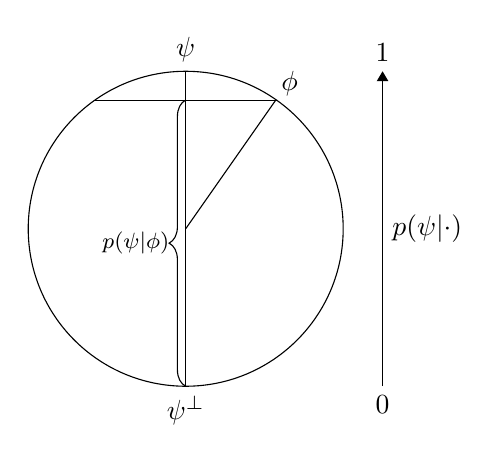
\begin{tikzpicture}[scale = 1, >=Triangle]
		\draw (0,0) circle (2);
		\node at (0,-2) [below] {$\psi^{\perp}$};
		\node at (0,2) [above] {$\psi$};
		\node at ($(0,0)!0.78!(1.4,2)$) [above right]  {$\phi$};
		\draw (0,-2) -- (0,2);
		\draw (0,-2) -- (0,2);
		\begin{scope}
			\clip(0,0) circle (2);
			\draw (0,0) -- (1.4,2);
			\draw (1.4,1.634) -- (-1.4,1.634);
		\end{scope}
		\draw[decorate,decoration={brace, amplitude = 6pt, raise = 0pt}] (0,-2) -- (0,1.634) node[midway, xshift = -18pt]{\footnotesize $p(\psi | \phi)$};
		\draw [->] (2.5,-2) node[below] {$0$} -- node[right] {$p(\psi | \cdot )$} (2.5,2) node[above] {$1$};
	\end{tikzpicture}
	\caption{Recovering the Born rule as an affine function of the ensemble space.}\label{rp-qm-geometricConditionalProbability}
\end{figure}
\end{proof}

\section{Conclusion}

Once we identify the space of ensembles with the ones given by the density operators, assuming the Born rule is equivalent to assuming the von Neumann entropy. The only extra requirement is the consistency between mutual exclusivity as defined over the conditional probability (i.e. $\psi$ and $\phi$ are mutually exclusive if and only if preparing one gives zero probability of having prepared the other) or over the entropy (i.e. $\phi$ and $\psi$ are mutually exclusive if and only if the entropy of their mixture is the Shannon entropy).
	
\end{document}